\chapter{Conclusion}
\label{conclusion}

In this thesis we investigated if it would be feasible to implement a provenance-based recommender system for recommending scientific datasets and pipelines given the other. We focused on the neuroimaging datasets and pipelines available in Canadian Open Neuroscience Platform (CONP) as of October 2020. For our recommender approach, we needed the provenance records generated in pipeline execution processes, however, there have been 2688 pairs of pipeline-datasets for execution. Therefore, we recruited 13 experts among graduate students, software developers and data engineers at the CONP and sent them a two phase survey to predict the execution outcome of all pipeline-dataset pairs which they have knowledge for both pipeline and dataset. Then we executed only the pipeline-dataset pairs for which at least one expert predicted a successful execution. All the generated provenance records are available at \url{https://github.com/big-data-lab-team/paper-pipelines-datasets-recommender/tree/main/data/}. Moreover, we have contributed to the web interface of CONP portal and uploaded all the provenance records there to be accessible on a dashboard, Figure~\ref{fig:dashProvenance}, so that users can search for any available combination of executed pipeline-dataset pairs and see the actual provenance records by clicking on their status, Figure~\ref{fig:execRecord} shows the provenance record for processing a file in `SIMON' dataset by `fsl\_bet' pipeline whith successful execution outcome (`exit-code' = 0).

\begin{figure*}
    \centering
    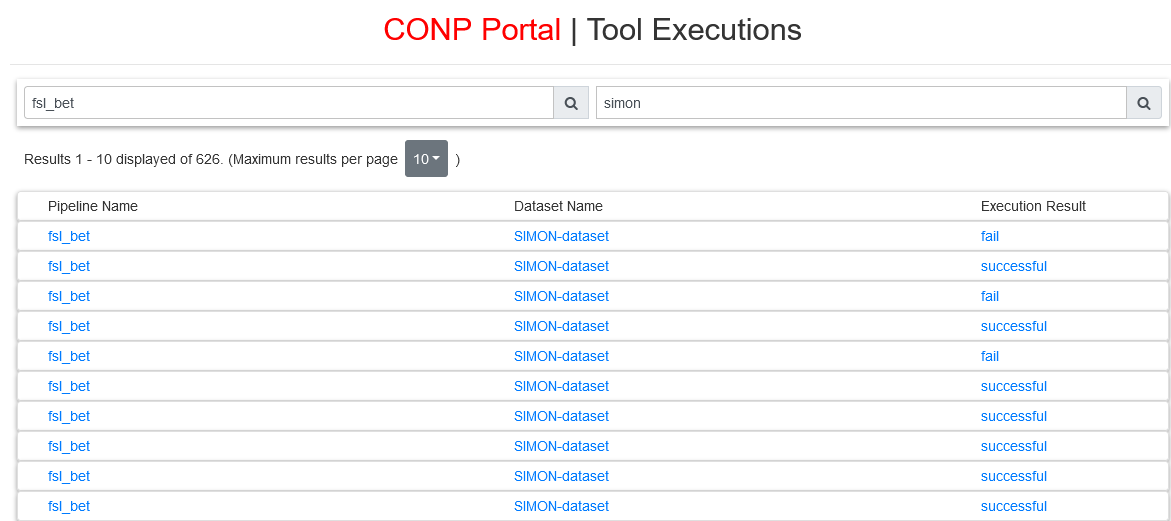
\includegraphics[width=\textwidth,height=\textheight,keepaspectratio]{figures/executiondashboard.png}
    \caption{Dashboard of Provenance Records integrated in CONP portal}
    \label{fig:dashProvenance}
\end{figure*}

\begin{figure*}
    \centering
    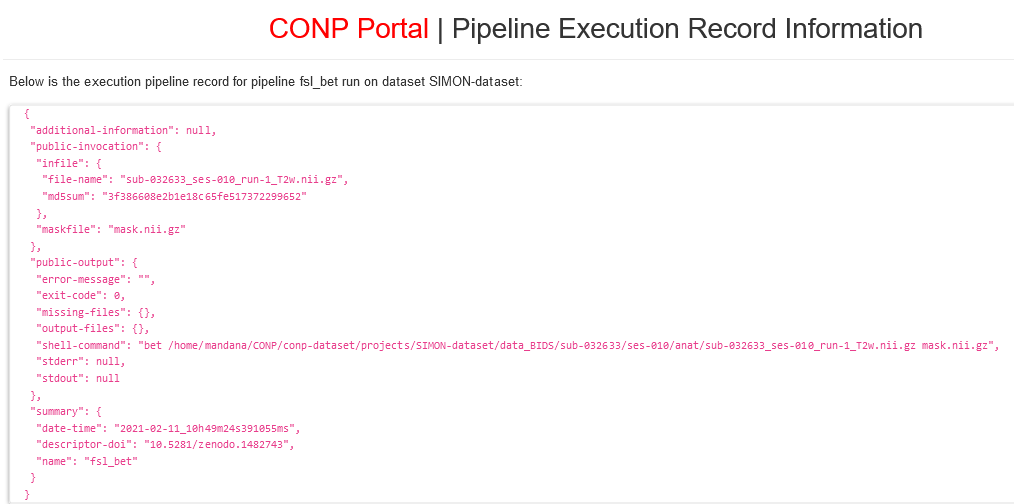
\includegraphics[width=\textwidth,height=\textheight,keepaspectratio]{figures/execRecord.png}
    \caption{One of the generated provenance records (JSON object)}
    \label{fig:execRecord}
\end{figure*}

From the outcome of these executions we filled the pipeline execution matrix ,Figure~\ref{fig:execution_matrix}, as the utility matrix for our recommender approach. Then, we applied Alternative Least Square model, which implements latent-factor model in Collaborative Filtering recommendation approach, on this matrix. We evaluated this model by applying 10-fold cross validation on the
pipeline execution matrix and varying the threshold for rounding the generated values to 1 (failed execution) or 2 (successful execution). Therefore, by creating the Receiver Operating Characteristic
(ROC) curve we got the area under curve (AUC) as $0.83$. We also evaluated the experts' predictions by applying varying thresholds on the fraction of experts predicting successful execution and got AUC = $0.63$ for the corresponding ROC curve which indicates that our system outperforms human experts' recommendations. 

There might be a several reasons why our system has a better performance than experts recommendations (predictions). There are many technical details that usually are ignored or neglected by the experts such as type compatibility of pipeline and dataset, pre-processing requirements for the pipelines, and availability and accessibility of the data at that time are some the reasons. Moreover, the good performance of our system could be expected to some extent since the pipeline execution matrix is not a random one and there are some sort structural patterns which helps the model having better accuracy.

Among the possible future works for this project, the most highlighted one is increasing the number of provenance records. These provenance records would be either uploaded by public users to a repository for CONP usage only or to distributed repositories which CONP would be responsible to collect them. Therefore, by having a large set of provenance records, more than one outcome for each pipeline-dataset pair, it might be required to change the recommendation approach for implicit feedback data. 
Since there would not be any limitation or range for the number of provenance records per pair, if the approach is going to focus on the number of executions per pair, the feedback data will not be explicit and it will be required to use collaborative filtering for implicit feedback data~\cite{hu2008collaborative}.

There would be some points to consider in this case, focusing only on the number of (successful) executions per pair will not provide strong and rational enough recommendations. For instance, some pipelines are simpler to use and mostly will be executed successfully, such as `fsl-bet', also accessing to some datasets is more straightforward than others, this leads to higher number of provenance records for specific pipeline-dataset pairs while they will not necessarily provide the best recommendations. It is important to consider the different factors: How many (successful) executions per pair? What fraction of all executions per pair is successful? How frequently the pipeline or dataset is used among all pipelines and datasets? What is the subtraction of successful and failed executions per pair? For considering these different factors, one possible approach can be an ensemble of utility matrices (one per factor) resulting a set of recommendation lists for each pair, then the final list can be the union of all these recommendations for each pair.

We are integrating the current version of this recommender system to the CONP portal and it will provide a full operational recommender system based on available provenance records. This system is supposed to work with the publicly uploaded provenance records on the CONP portal and provide a list of highly recommended pipelines for a dataset in each dataset card and the highly recommended datasets for in each pipeline card. Figure~\ref{fig:mockup} represents the sample dataset recommendations for `fsl-bet' pipeline.

\begin{figure*}
    \centering
    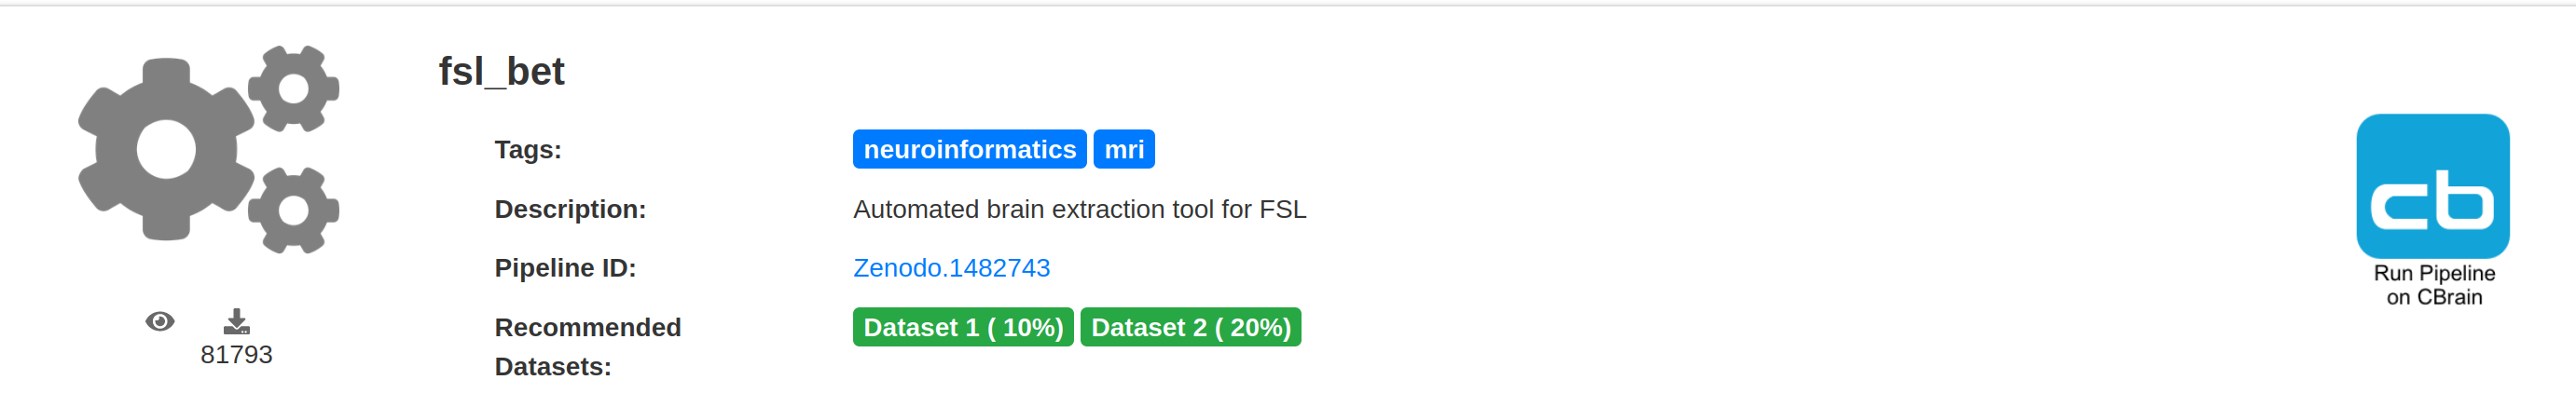
\includegraphics[width=\textwidth]{figures/mockup.png}
    \caption{The mock-up for the recommender system to be integrated in CONP portal}
    \label{fig:mockup}
\end{figure*}